\chapter{Nociones Preliminares}
\label{Nociones Preliminares}


En este capítulo se exhiben los principales conceptos sobre las áreas de base que conforman este trabajo, estas son: Workflow y Workflow Management System (WFMS), Web Services (WS), el lenguaje WSDL, el Protocolo de Acceso a Objetos Simple (Simple Object Access Protocol - SOAP) y desarrollo dirigido por modelos.

\section{Workflows}
\label{Workflows}

Uno de los problemas que se encuentra habitualmente en el desarrollo de aplicaciones para Negocios, es que las tareas o procesos que se desarrollan en el entorno laboral de las mismas quedan inmersos en el código de la aplicación que resuelve la problemática del Negocio. Está claro que la gran mayoría de los usuarios no tienen conocimiento de estas tareas, las mismas están ocultas a sus ojos y se realizan automáticamente. El hecho de realizar cambios en dichas tareas o procesos resulta muy costoso, y es muy factible que dichos cambios redunden en realizar nuevamente la aplicación.\\

Una buena solución al problema anterior es separar los procedimientos y asociarlos a los Workflows realizados dentro de la Negocio. El Workflow se relaciona con la automatización de los procedimientos donde los documentos, la información o tareas son pasadas entre los participantes del sistema de acuerdo a un conjunto de reglas previamente establecidas. El fin de lo anterior es llegar a culminar una meta común impuesta por la Negocio.\\

Se puede ver al Workflow como un conjunto de métodos y tecnologías que ofrece las facilidades para modelar y gestionar los diversos procesos que ocurren dentro de una Negocio. El Workflow es el último, de una gran línea de facilidades propuestas en respuesta de las exigencias de las organizaciones, las cuales apuntan a poder reaccionar tan rápido como sea posible ante la frenética demanda de la competición. Además, permite automatizar diferentes aspectos del flujo de la información: rutear los trabajos en la secuencia correcta, proveer acceso a datos y documentos, y manejar ciertos aspectos de la ejecución de un proceso.\\

La diversidad de procesos que puede haber en una organización lleva a pensar en la existencia de diferentes tipos de software de Workflow. El Workflow ofrece a un negocio la posibilidad de automatizar sus procesos, reducir costos, y mejorar servicios, obvios beneficios. Organizaciones que no hayan evaluado esta tecnología podrían encontrarse con desventajas en un futuro.

\section{Workflow Management Coalition}
\label{Workflow Management Coalition}

La WfMC es una agrupación compuesta por compañías, vendedores, organizaciones de usuarios, y consultores. El objetivo de esta agrupación es ofrecer una forma de ``diálogo'' común a todos. De esta forma las diferentes herramientas que se implementen en esta área podrán tener cierto nivel de interoperabilidad, es decir, podrán comunicarse entre ellas para poder realizar las distintas tareas involucradas en un sistema de Workflow.\\

De acuerdo a la definición de la WfMC, en un WFMS existen dos actividades bien diferenciadas. Por un lado, se tiene la definición del Workflow que implementa el proceso de negocio, lo que se denomina modelado del Workflow. Este modelado consiste en la definición de un conjunto de actividades relacionadas y un conjunto de criterios que indican el comienzo y la finalización del proceso. Además, se definen sus componentes e información adicional sobre cada actividad tal como participantes, invocación de aplicaciones, datos, etc. En el modelado participan los siguientes elementos:

\begin{itemize}
	\item Proceso de Negocio: un conjunto de uno o más procedimientos o actividades que colectivamente realizan un objetivo o política global de una organización.
	
	\item Definición del Proceso: la representación de un proceso de negocio en una forma que soporta la manipulación automática. La definición consiste de un conjunto de actividades y sus relaciones.
	
	\item Actividades: la descripción de un trozo de trabajo que forma un paso lógico dentro de un proceso.
	
	\item Actividades Automáticas: las que soportan la automatización por computadora. 
	
	\item Actividades Manuales: las que no soportan la automatización por computadora y por lo tanto quedan fuera de alcance del WFMS.
\end{itemize}

Por un lado, está la ejecución de dicho modelo. La ejecución del Workflow en un WFMS consiste en la creación, manipulación y destrucción de instancias de proceso, que representan al Workflow de acuerdo a la especificación realizada en el modelado. Cada instancia de proceso tendrá una identidad visible externamente y un estado interno que representa su progreso hacia la finalización y su estado con respecto a las actividades que lo componen. Cada vez que la ejecución de un proceso implique la invocación de una actividad, se crea una instancia de actividad que la representa. Dicha instancia se encarga de ejecutar las acciones asignadas, accediendo a los datos que sean necesarios e invocando la aplicación externa correspondiente, si así lo requiere la actividad. Los elementos que participan en la ejecución son:

\begin{itemize}
	\item Instancias de Proceso: representan un proceso simple, incluyendo sus datos asociados.
	
	\item Instancias de Actividad: representan una actividad dentro de una instancia de proceso.
	
	\item Ítem de Trabajo: es la representación de una tarea a ser procesada por un participante del Workflow, en el contexto de una actividad dentro de una instancia de proceso. Cada tarea es un conjunto de acciones manejadas como una sola unidad. Generalmente son desempeñadas por una única persona dentro de los roles que pueden realizar dicha tarea. Las tareas surgen del análisis del Workflow, donde se define por quienes deben ser ejecutadas.
	
	\item Invocación de Aplicaciones: es la representación de las aplicaciones del Workflow que son invocadas por el WFMS para automatizar una actividad.
\end{itemize}

\section{Invocación de Aplicaciones Externas a un WFMS según el Modelo de referencia de la WfMC}
\label{Invocación de Aplicaciones Externas a un WFMS según el Modelo de referencia de la WfMC}

La WfMC ha estandarizado la automatización de los procesos de negocio. Dicho estándar define un marco genérico para la construcción de WFMS, permitiendo la interoperabilidad entre ellos y con otras aplicaciones. Entonces, el modelo de referencia de Workflow fue desarrollado desde estructuras genéricas de aplicaciones de Workflow, identificando las interfaces con estas estructuras, de forma de permitir a los productos comunicarse a distintos niveles. Todos los sistemas de Workflow contienen componentes genéricos que interactúan de forma definida. Para poder tener cierto nivel de interoperabilidad entre los diversos productos de Workflow, es necesario definir un conjunto de interfaces y formatos para el intercambio de datos entre dichos componentes \cite{WfMC09}.\\

En la figura \ref{fig:Interfaces del Modelo de Referencia} se muestran las distintas interfaces y componentes que se pueden encontrar en la arquitectura del Workflow.

\begin{figure}[!h] 
	\begin{center}
		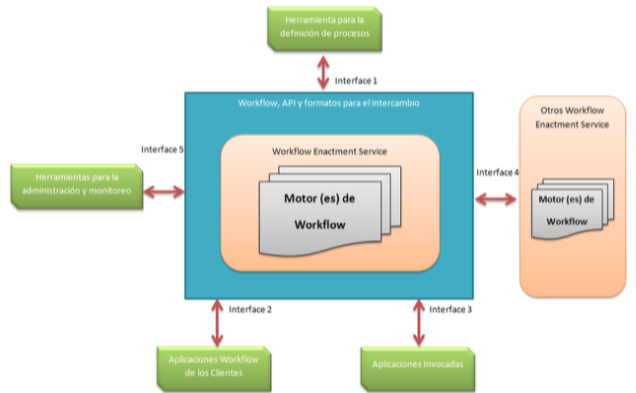
\includegraphics [scale=0.50]{imagenes/Interfaces_del_Modelo_de_Referencia.png}
	\end{center}
	\caption{Interfaces del Modelo de Referencia.}
	\label{fig:Interfaces del Modelo de Referencia}
\end{figure} 

En el modelo adoptado hay una separación entre los procesos y el control de la lógica de las actividades. Esta lógica está dentro del Workflow Enactment Service. Esta separación permite la integración de las diversas herramientas con una aplicación particular. La interacción del Enactment Service con los recursos externos se da por una de las dos interfaces siguientes:

\begin{itemize}
	\item La interface de las Aplicaciones de los Clientes, a través de la cual el Motor de Workflow interactúa con el manejador de la Worklist, responsable de organizar el trabajo por intermedio de un recurso de usuario. Es responsabilidad del manejador del Worklist elegir y hacer progresar cada elemento de la lista de trabajo (Worklist).
	
	\item La interfaz de las Aplicaciones Invocadas, la cual le permite al motor de Workflow activar una herramienta para realizar una actividad particular. Esta interface podría ser basada en un servidor, es decir no existe la interacción con el usuario.
	
\end{itemize}

El Motor de Workflow (Workflow Engine) es el software que provee el control del ambiente de ejecución de una instancia de Workflow. Típicamente dicho software provee facilidades para:

\begin{itemize}
	\item Interpretación de la definición de procesos.
	
	\item Control de las instancias de los procesos: creación, activación, terminación, etc. Navegación entre actividades.
	
	\item Soporte de interacción con el usuario.
	
	\item Pasaje de datos al usuario o a aplicaciones.
	
	\item Invocación de aplicaciones externas.
\end{itemize}

Por otra parte, las WAPI pueden ser vistas como un conjunto de llamadas API (Application Programming Interface) y funciones de intercambio de datos soportadas por el Workflow Enactment Service. Las APIs son un conjunto de llamadas a funciones de software que permiten a las aplicaciones acceder a funciones de un programa. Las WAPI permiten la interacción del Workflow Enactment Service con otros recursos y aplicaciones.

\section{Web Service}
\label{Web Service}

El término Web Service se utiliza muy a menudo hoy en día, aunque no siempre con el mismo significado. Los conceptos y tecnologías subyacentes de los WS's son en gran medida independientes de la forma en que puedan ser interpretadas. Las definiciones existentes para el concepto de WS, van desde la muy genérica y con todo incluido a la muy específica y restrictiva.\\

Entonces, se puede comenzar por definir a un WS como un estándar de comunicación entre procesos y/o componentes, diseñado para ser multiplataforma y multilenguaje, es decir, no importa en qué lenguaje esté programado un WS como ser Visual Basic, C\# o Java, o en qué plataforma esté corriendo, ya sea Windows, UNIX o Linux éstos serán accesibles y utilizables por otras aplicaciones desarrolladas en otras plataformas o lenguajes de programación. Es decir, diversas aplicaciones de software desarrolladas en lenguajes de programación diferentes, y ejecutadas sobre cualquier plataforma, pueden utilizar los WS's para intercambiar datos tanto en redes locales como en Internet. Esta interoperabilidad se consigue mediante la adopción de estándares abiertos. Las organizaciones, esencialmente la W3C, son los comités responsables que se encargan de la arquitectura y la reglamentación de los WS's.\\

Precisamente la W3C define a los WS's como ``Aplicaciones de software identificadas mediante una URI (Uniform Resource Identifier), cuyas interfaces (y uso) son capaces de ser definidas, descritas y descubiertas mediante artefactos XML, y soportar interacciones directas con otras aplicaciones software usando mensajes basados en XML y protocolos basados en Internet''.\\

En el mundo de los WFMS, tanto los usuarios como los administradores de Workflow usualmente requieren la utilización de aplicaciones externas para desarrollar sus tareas, por ejemplo, aplicaciones que le permitan utilizar servicios de e-mail, fax, realizar la administración de sus documentos, u otras aplicaciones propias del usuario como obtener fechas, climas o cálculos matemáticos provistos desde la web.\\

Por otra parte, los WS's pueden ser agrupados según las funcionalidades que ofrecen en: de Información de negocios (pronóstico del tiempo, calendario, noticias, chequeo de crédito de una tarjeta, subastas, cotizaciones de acciones, planificación de vuelos, etc.); de Transacciones (reservas aéreas, acuerdos para rentar un auto, orden de compra, gestión de una cadena de suministro, etc.); o de Externalización de procesos de negocio (vínculos comerciales a nivel de Workflow, etc.).\\

Los WS's se describen en términos de sus operaciones y de los mensajes de entrada y salida de cada una de esas operaciones que provee. Tales definiciones se expresan en el lenguaje de marcado extensible XML (Extensible Markup Language) \cite{XML}, usando un lenguaje de descripción de WS's: WSDL (Web Service Description Language)\cite{WSDL2.0-0} \cite{WSDL2.0-1}. La noción de describir un WS independientemente de la tecnología en la cual ha sido implementado es robustamente capturada en este lenguaje. WSDL especifica claramente la ubicación del servicio junto con las operaciones que necesitan ser invocadas, los parámetros que deben pasarse, los tipos de datos de cada parámetro, y los distintos formatos de mensajes y tipos.\\ 

Así, el uso de protocolos estándares como WSDL en el contexto de los WS's es necesario sin excepciones para poder lograr la interoperabilidad en estos ambientes heterogéneos, con independencia del sistema operativo, el lenguaje de programación, etc. Otros estándares que se utilizan al hablar de WS's son:
\begin{itemize}
	
	\item \textbf{Protocolo HTTP (Hiper Text Transport Protocol) \cite{HTTP}:}
	 HTTP es la abreviatura de HyperText Transfer Protocol, HTTP es el protocolo utilizado por la World Wide Web. HTTP define cual es el formato de los mensajes, y cómo se transmiten los mismos. HTTP es un protocolo sin estado, se lo llama así  ya que cada comando se ejecuta de forma independiente, sin ningún conocimiento de los comandos que vinieron antes que él. Esta es la razón principal por la que es difícil de implementar sitios Web que reaccionan de forma inteligente a la entrada del usuario. Esta deficiencia de HTTP está siendo abordada en una serie de nuevas tecnologías, incluyendo ActiveX, Java, JavaScript y las cookies.
	
	\item \textbf{Protocolo SOAP (Simple Object Access Protocol) \cite{SOAP}: }
	SOAP (Simple Object Access Protocol) es el protocolo base de los WS's. Este protocolo está basado en XML y no se encuentra atado a ninguna plataforma o lenguaje de programación. A su vez, también es el protocolo más aceptado por la mayoría de las plataformas. 
	Si bien SOAP es un protocolo, éste no es exactamente un protocolo de comunicación entre mensajes como lo es el HTTP, por ejemplo. Básicamente, SOAP son documentos XML y necesitaremos utilizar algún otro protocolo para la transmisión de estos documentos como ser el protocolo HTTP o cualquier otro protocolo de comunicación capaz de transmitir textos. En la figura \ref{fig:Composición del protocolo SOAP} podemos ver como SOAP esa compuesto.
	



\begin{figure}[!h] 
	\begin{center}
		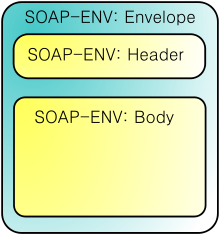
\includegraphics [scale=0.50]{imagenes/Composicion_del_protocolo_SOAP.png}
	\end{center}
	\caption{Composición del protocolo SOAP.}
	\label{fig:Composición del protocolo SOAP}
\end{figure} 

	\item \textbf{UDDI (Universal Description, Discovery and Integration) \cite{UDDI}:} Se utiliza para el registro y la localización de cualquier WS. Se trata de un directorio o catálogo de WS's distribuido que permite que se listen, busquen y descubran este tipo de aplicaciones de software.
	UDDI tiene como objetivo ser accedido por los mensajes SOAP y dar paso a documentos WSDL.\\
\end{itemize}


Cada uno de estos protocolos se asocian a una capa, las cuales en conjunto, definen la infraestructura de los WS's.\\


\begin{itemize}
	\setlength{\itemindent}{.5in}
	\item[HTTP:] Corresponde La capa de transporte utilizada para el envío de la información;
	\item[SOAP:] Corresponde a la capa de mensajes.
	\item[WSDL:] Corresponde a la capa de descripción.
	\item[UDDI:] Corresponde a la capa de procesos que se encargan de la publicación, descubrimiento, composición, orquestación, desarrollo e integración de WS's. Al desaparecer los registos UDDI publicos, esta tesis plantea una solución usando una base conocida de WS's.
\end{itemize}

\subsection{El lenguaje WSDL}
\label{El lenguaje WSDL}

WSDL (Web Service Description Language) es el lenguaje de especificación utilizado para definir los WS's. Se trata de un documento XML que se utiliza para describir los mensajes SOAP y cómo estos mensajes son intercambiados. Es decir, supongamos que creamos un WS y queremos que otras aplicaciones lo utilicen, las otras aplicaciones deberán acceder a un documento WSDL en donde podrán conocer los métodos que expone nuestro WS y cómo acceder a ellos, es decir, cuáles son los nombres de los métodos y qué tipos de parámetros espera cada uno de ellos. Entonces, en este sentido, cualquier documento WSDL permite proveer información acerca de la ubicación de cierto WS y su interfaz. Así, con esta información respecto a la descripción y especificación del WS, el usuario sabrá básicamente cómo llevar a cabo la interacción con el servicio.\\

Hay que tener en cuenta que todo documento WSDL separa la descripción de un servicio en dos partes \cite{WSA}. Dentro de cada una de estas partes, se utilizan un número de constructores que promueven la reusabilidad de la descripción y permiten separarla de los detalles de diseño. Una de ellas es la interfaz abstracta, la cual describe las operaciones soportadas por el servicio, los parámetros de la operación y los tipos de datos abstractos. Esta descripción es completamente independiente de la dirección de red concreta, el protocolo de comunicación o las estructuras de datos concretas del servicio. La otra parte es la implementación concreta, la cual liga la interfaz abstracta a una dirección de red, protocolo y estructuras de datos concretas. WSDL provee toda esta información a través de elementos XML. \\

Por un lado, en la Interfaz Abstracta los dos elementos a definir son:\\

\begin{enumerate}[1.]
	\item \textbf{types:} provee la definición de los tipos de datos utilizados para describir los mensajes a intercambiar, sus operaciones los parámetros de entrada o salida de cada operación.
	
	\item \textbf{interface:} describe la secuencia de mensajes que el servicio envía o recibe.
\end{enumerate}


Y por el otro, los dos elementos a definir en la implementación concreta son:

\begin{enumerate}[1.]
	\item \textbf{binding:} define los detalles de implementación concretos del servicio.
	
	\item \textbf{service:} se usa para asociar un binding con el URL donde está realmente el servicio (endpoint).
\end{enumerate}

Entonces cualquier documento WSDL especifica tanto la definición como una descripción del WS que representa. Pero también define los dos componentes principales de estos, es decir, sus características funcionales y sus características no funcionales.  La descripción funcional se refiere a las características operacionales que definen el comportamiento general de un WS. En otras palabras, define los detalles de cómo es invocado el servicio, su ubicación, etc. Esta descripción focaliza en los detalles de la sintaxis de los mensajes y cómo configurar los protocolos de red para enviar estos mensajes. Y el otro componente, la descripción no funcional, se concentra en las características de calidad (QoS) del WS.


\subsection{Características de Calidad de los Web Services}
\label{Características de Calidad de los Web Services}

Los requerimientos de un WS no deben focalizar solamente en las propiedades funcionales del mismo, sino que también se deben concentrar en describir el ambiente en el que se desarrolla, es decir, describir las capacidades no funcionales o QoS del servicio \cite{W3C03-QoS}. Cada servicio puede ofrecer diversas opciones de características no funcionales basadas en los requerimientos técnicos como: disponibilidad, performance y escalabilidad, políticas de seguridad y privacidad, etc., todas las cuales deben ser descriptas.

Los elementos clave que se tienen en cuenta para soportar las QoS en el mundo de los WS's son:
\begin{itemize}
	\item \textbf{Rendimiento o throughput:} Número de requerimientos de WS's atendidos en un período de tiempo dado.
	
	\item \textbf{Tiempo de Respuesta:} Tiempo esperado entre que se envía un requerimiento y se recibe una respuesta.
	
	\item \textbf{Latencia:} Tiempo entre que un requerimiento de un servicio arriba y el requerimiento comienza a ser atendido.
	
	\item \textbf{Tiempo de Ejecución:} Es el tiempo que necesita un WS para procesar su secuencia de actividades.
	
	\item \textbf{Tiempo de Transacción:} Representa el tiempo que transcurre mientras el WS está completando una transacción.
	
	\item \textbf{Disponibilidad:} Probabilidad de que el WS esté disponible.
	
	\item \textbf{Fiabilidad:} Habilidad de un servicio para funcionar correcta y consistentemente y proveer la misma calidad a pesar de las fallas en la red o el sistema.
	
	\item \textbf{Precisión:} Radio de error producido por un servicio.
	
	\item \textbf{Robustez:} Grado en el cual un servicio puede funcionar correctamente en presencia de entradas inválidas, incompletas o conflictivas.
	
	\item \textbf{Reputación:} Medida de la reputación otorgada al servicio por el usuario final.
	
\end{itemize}

Tradicionalmente, las QoS se miden por el grado en el cual las aplicaciones, sistemas, redes y otros elementos de Internet soportan la disponibilidad de los servicios a un nivel requerido de performance, en todos los accesos y condiciones de descarga. En el contexto de los WS's, las QoS se pueden ver como la capacidad de ofrecer garantía sobre un conjunto de características cuantitativas, referidas específicamente a los aspectos no funcionales de los servicios. Estas características son un requerimiento necesario para entender el comportamiento subyacente del servicio de manera tal que otras aplicaciones y servicios puedan invocarlos y ejecutarlos como parte de su proceso de negocio.\\

En este trabajo se propone una forma de incorporar las QoS en los WS's a partir de la necesidad de tenerlas en cuenta a la hora de optimizar el proceso de selección del WS más adecuado. Esta incorporación ofrece importantes beneficios, tanto para los usuarios como los proveedores. A los usuarios les permite expresar sus necesidades y utilizar el WS que mejor se ajusta sus necesidades, mientras que los proveedores pueden publicar mejor las capacidades de sus servicios y lucirse con las mismas.

\section{Desarrollo de software dirigido por modelos}
\label{Desarrollo de software dirigido por modelos}

El desarrollo de software dirigido por modelos surge como respuesta a los principales problemas que actualmente tienen las compañías de desarrollo de software, por un lado, para gestionar la creciente complejidad de los sistemas que construyen y mantienen, y por otro para adaptarse a la rápida evolución de las tecnologías software.

En primer lugar, se usan modelos para representar tanto los sistemas como los propios artefactos del software. Cada modelo trata un aspecto del sistema, que puede ser especificado a un nivel más elevado de abstracción y de forma independiente de la tecnología utilizada. Este hecho permite que la evolución de las plataformas tecnológicas sea independiente del propio sistema, disminuyendo así sus dependencias.

En segundo lugar, se consigue también proteger gran parte de la inversión que se realiza en la informatización de un sistema, pues los modelos son los verdaderos artífices de su funcionamiento final y, por tanto, no será necesario empezar desde cero cada vez que se plantee un nuevo proyecto o se desee realizar algún tipo de mantenimiento sobre el producto.

En tercer lugar, en MDA los modelos constituyen la propia documentación del sistema, disminuyendo considerablemente el coste asociado y aumentando su mantenibilidad, puesto que la implementación se realiza de forma automatizada a partir de la propia documentación.

\subsection{Modelos}
\label{Modelos}

De forma sencilla podríamos definir un modelo como una abstracción simplificada de un sistema o concepto del mundo real. Un modelo de un cierto <X> es una especificación o descripción de ese <X> desde un determinado punto de vista, expresado en un lenguaje bien definido y con un propósito determinado.\\

Según Bran Selic, uno de los fundadores del MDD y pionero en el uso de sus técnicas, los modelos deberían ser:
\begin{itemize}
	\item \textbf{Adecuados:} Construidos con un propósito concreto, desde un punto de vista determinado y dirigidos a un conjunto de usuarios bien definido.
	
	\item \textbf{Abstractos:} Enfatizan los aspectos importantes para su propósito a la vez que ocultan los aspectos irrelevantes.
	
	\item \textbf{Comprensibles:} Expresados en un lenguaje fácilmente entendible para sus usuarios.
	
	\item \textbf{Precisos:} Representan fielmente al objeto o sistema modelado.
	
	\item \textbf{Predictivos:} Pueden ser usados para responder preguntas sobre el modelo e inferir conclusiones correctas.
	
	\item \textbf{Rentables:} Han de ser más fáciles y baratos de construir y estudiar que el propio sistema.
\end{itemize}

Bran Selic también señala las principales funciones que los modelos deberían tener en el ámbito de la ingeniería del software:

\begin{itemize}
	\item \textbf{Comprender el sistema}
		\begin{itemize}
			\item La estructura, el comportamiento y cualquier otra característica relevante de un sistema y su entorno desde un punto de vista dado.
			
			\item Separar adecuadamente cada uno de los aspectos, describiendolos al nivel conceptual adecuado.
		\end{itemize}
	\item \textbf{Servir de mecanismo de comunicación}
		\begin{itemize}
			\item Con los distintos tipos de stakeholder del sistema (desarrolladores, usuarios finales, personal de soporte y mantenimiento, etc.).
			
			\item Con las otras organizaciones (proveedores y clientes que necesitan comprender el sistema a la hora de interoperar con él).
		\end{itemize}	
	\item \textbf{Validar el sistema y su diseño}
		\begin{itemize}
			\item Detectar errores, omisiones y anomalías en el diseño tan pronto como sea posible (cuanto antes se detecten, menos cuesta corregirlos).
			
			\item Razonar sobre el sistema, infiriendo propiedades sobre su comportamiento (en caso de modelos ejecutables que puedan servir como prototipos).
			
			\item Poder realizar análisis formales sobre el sistema.
		\end{itemize}		
	\item \textbf{Guiar la implementación}
		\begin{itemize}
			\item Servir como ``planos'' para construir el sistema y que permitan guiar su implementación de una forma precisa y sin ambigüedades.
			
			\item Generar, de la forma más automática posible, tanto el código final como todos los artefactos necesarios para implementar, configurar y desplegar el sistema.
		\end{itemize}	
	
\end{itemize}

\subsection{Metamodelos}
\label{Metamodelos}

Un metamodelo es un modelo que especifica los conceptos de un lenguaje, las relaciones entre ellos y las reglas estructurales que restringen los posibles elementos de los modelos válidos, así como aquellas combinaciones entre elementos que respetan las reglas semánticas del dominio.
De esta forma, cada modelo se escribe en el lenguaje que define su metamodelo (su lenguaje de modelado), quedando establecida la relación entre el modelo y su metamodelo por una relación de “conformidad” (y diremos que un modelo es “conforme a” un metamodelo). Esta relación se puede observar en la figura \ref{fig:Relación modelo metamodelo}.

\begin{figure}[!h]
	\begin{center}
		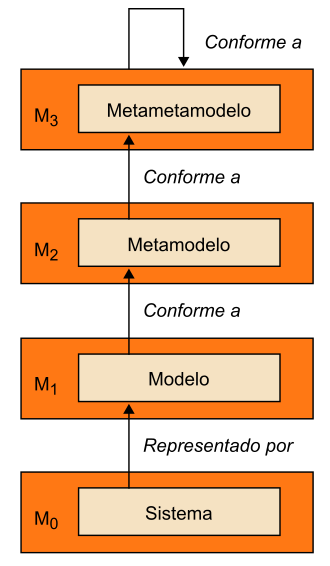
\includegraphics [scale=0.40]{imagenes/Relacion_modelo_metamodelo.png}
	\end{center}
	\caption{Relación modelo metamodelo.}
	\label{fig:Relación modelo metamodelo}
\end{figure} 

\subsection{Terminología}
\label{Terminología}

La comunidad utiliza en la actualidad un conjunto de acrónimos referidos a diferentes enfoques relacionados con la ingeniería del software que usa modelos como elementos clave de sus procesos: MDD, MBE, MDA, etc. Aunque algunos de ellos ya se han mencionado en secciones anteriores, en este apartado trataremos de aclarar estos conceptos y las diferencias entre ellos.\\

MDD (model-driven development) es un paradigma de desarrollo de software que utiliza modelos para diseñar los sistemas a distintos niveles de abstracción, y secuencias de transformaciones de modelos para generar unos modelos a partir de otros hasta generar el código final de las aplicaciones en las plataformas destino \cite{3}.

MDA (model-driven architecture) es la propuesta concreta de la OMG para implementar MDD, usando las notaciones, mecanismos y herramientas estándares definidos por esa organización \cite{5}.\\

Los estándares que la OMG ofrece para realizar MDA incluyen, entre otros:

\begin{itemize}
	\item UML (unified modeling language) como lenguaje de modelado.
	\item MOF (meta-object facility) como lenguaje de metamodelado.
	\item OCL (object constraint language) como lenguaje de restricciones y consulta de modelos.
	\item QVT (query-view-transformation) como lenguaje de transformación de modelos.
	\item XMI (XML metadata interchange) como lenguaje de intercambio de información.
\end{itemize}

MDE (model-driven engineering) es un paradigma dentro de la ingeniería del software que aboga por el uso de los modelos y las transformaciones entre ellas como piezas clave para dirigir todas las actividades relacionadas con la ingeniería del software.\\

MBE (model-based engineering) es un término general que describe los enfoques dentro de la ingeniería del software que usan modelos en algunos de sus procesos o actividades.\\

BPM (business process modeling) es una rama del model-based engineering que se centra en el modelado de los procesos de negocio de una empresa u organización, de forma independiente de las plataformas y las tecnologías utilizadas.\\

Architecture-driven modernization (ADM) es una propuesta de la OMG para implementar prácticas de ingeniería inversa utilizando modelos.\\

Model driven-interoperability (MDI) es una iniciativa para implementar mecanismos de interoperabilidad entre servicios, aplicaciones y sistemas usando modelos y técnicas de MBE.\\

En la figura \ref{fig:Relacíon entre los contextos de MDE, MDD y MDA} se puede observar la relación entre los contextos de MDE, MDD, MDA.

\begin{figure}[!h] 
	\begin{center}
		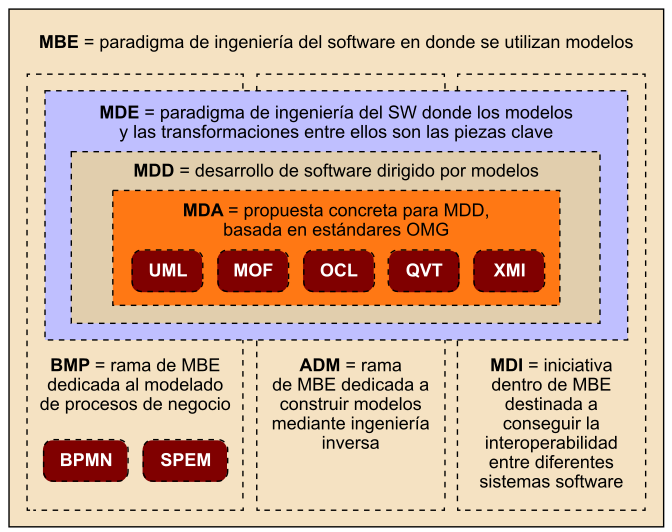
\includegraphics [scale=0.50]{imagenes/Relacion_MDE_MDD_MDA.png}
	\end{center}
	\caption{Relación entre los contextos de MDE, MDD y MDA.}
	\label{fig:Relacíon entre los contextos de MDE, MDD y MDA}
\end{figure} 

\subsection{Transformaciones de modelos}
\label{Transformaciones de modelos}

\subsubsection*{La necesidad de las transformaciones de modelos} 
\label{La necesidad de las transformaciones de modelos} 

Las transformaciones de modelos proporcionan los mecanismos que permiten especificar el modo de producir modelos de salida a partir de modelos de entrada.\\
El concepto de transformación en el mundo de la informática no es nuevo, de hecho, las transformaciones son algo fundamental en la ingeniería del software, pudiendo verse la computación como un proceso de transformación de datos.

Entre las aplicaciones de las transformaciones de modelo en el ámbito de MDE nos encontramos:

\begin{itemize}
	\item Generación de modelos a más bajo nivel, y finalmente código, a partir de modelos a alto nivel.
	\item Sincronización y mapping entre modelos al mismo o diferentes niveles de abstracción.
	\item Creación de vistas basadas en queries sobre un sistema.
	\item Aplicación a la ingeniería inversa para obtener modelos a más alto nivel a partir de modelos a más bajo nivel.
\end{itemize}

\subsubsection*{Conceptos básicos}
\label{Conceptos básicos}

Las transformaciones de modelos pueden verse como programas que toman un modelo (o más de uno) como entrada y retornan otro modelo (o más de uno) como salida.\\
Generalmente, una transformación de modelos está formada por un conjunto de reglas de transformación, que son consideradas como las unidades de transformación más pequeñas. Cada una de las reglas describe cómo uno o más elementos del modelo origen son transformados en uno o más elementos del modelo destino.

La figura \ref{fig:Transformación de modelo} demuestra como se lleva a cabo una transformación de modelo.

\begin{figure}[!h] 
	\begin{center}
		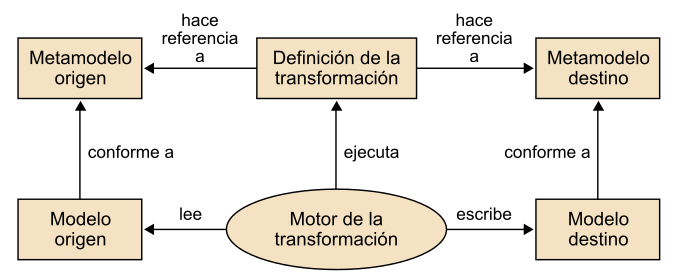
\includegraphics [scale=0.50]{imagenes/Transformacion_modelo.png}
	\end{center}
	\caption{Transformación de modelo.}
	\label{fig:Transformación de modelo}
\end{figure} 

\subsubsection*{Tipos de transformaciones}
\label{Tipos de transformaciones}

En MDE se describen diferentes tipos de transformaciones entre modelos, dependiendo de varios criterios:

\begin{enumerate}[a)]
    \item Nivel de abstracción de los modelos de entrada y salida.
    \begin{itemize}
		\item Transformaciones verticales. Relacionan modelos del sistema situados en distintos niveles de abstracción y pueden aplicarse tanto en sentido descendente como en sentido ascendente, siendo estos últimos el resultado de aplicar un proceso de ingeniería inversa.
		\item Transformaciones horizontales. Relacionan los modelos que describen un sistema desde un nivel de abstracción similar. Se utilizan también para mantener la consistencia entre distintos modelos de un sistema, es decir, garantizan que la información modelada sobre una entidad en un modelo es consistente con lo que se dice sobre dicha entidad en cualquier otra especificación situada al mismo nivel de abstracción.
    \end{itemize}
    \item Tipo de lenguaje que se utiliza para especificar las reglas. Se distingue entre lenguajes declarativos, imperativos o híbridos (si permiten ambos tipos de forma combinada).
    \item Atendiendo a la direccionalidad, nos encontramos con:
    \begin{itemize}
    	\item Transformaciones unidireccionales, las reglas se ejecutan en una sola dirección.
    	\item Transformaciones bidireccionales. En estas, las transformaciones se pueden aplicar en ambas direcciones .
    \end{itemize}
    \item Dependiendo de los modelos origen y destino:
    \begin{itemize}
    	\item Transformaciones exógenas. Los metamodelos origen y destino son distintos. Es el caso más común: se tiene un modelo de entrada y se obtiene el de salida a partir de él aplicando las reglas de la transformación. 
    	\item Transformaciones endógenas. Aquí, los metamodelos origen y destino son el mismo, se trata de las llamadas transformaciones in-place: las reglas de transformación se van aplicando sobre el propio modelo de entrada, de modo que este se va transformando hasta que no se puede aplicar ninguna regla más y el modelo de entrada pasa a ser el de salida.
    \end{itemize}
    \item Atendiendo al tipo de modelo destino:
    \begin{itemize}
    	\item Transformaciones modelo a modelo (M2M), las cuales generan modelos a partir de otros modelos.
    	\item Transformaciones modelo a texto (M2T), que generan cadenas de texto a partir de modelos. Son usadas, por ejemplo, para generar código y documentos.
    	\item Transformaciones texto a modelo (T2M), que generan modelos a partir de cadenas de texto.
    \end{itemize}
\end{enumerate}

\subsubsection*{Transformaciones de modelos en MDA}
\label{Transformaciones de modelos en MDA}

Una transformación de modelos es el proceso de convertir un modelo de un sistema en otro modelo del mismo sistema.\\

En esencia, una transformación establece un conjunto de reglas que describen cómo un modelo expresado en un lenguaje origen puede ser transformado en un modelo en un lenguaje destino.\\

Para definir una transformación entre modelos es necesario:
\begin{enumerate}[1.]
	\item Seleccionar el tipo de transformación y el lenguaje de definición de transformaciones a utilizar 
	\item Seleccionar la herramienta que nos permita implementar los modelos y las transformaciones de forma automática.	
\end{enumerate}

\section{QVT}
\label{QVT}

QVT es la propuesta del OMG para resolver el problema de la transformación de modelos. Se trata de un estándar para la definición de transformaciones sobre modelos MOF.  La especificación de QVT depende de otros dos estándares de la OMG como son MOF y OCL.\\

El lenguaje en sí define tres diferentes lenguajes de transformación: Relations, Core y Operational.\\

En la dimensión de la interoperabilidad se encuentran aquellas características que permiten a una herramienta que cumple el estándar QVT interopere con otras herramientas.\\
Concretamente, son cuatro:

\begin{itemize}
	\item La sintaxis ejecutable se traduce en una implementación que facilite la importación o lectura, y posterior ejecución de una sintaxis concreta que describa una transformación definida en el lenguaje dado por la dimensión del lenguaje.	 	 	 	
	\item XMI ejecutable dictamina que una implementación debe facilitar la importación o lectura, y posterior ejecución de una serialización XMI de una transformación que conforma con el metamodelo de MOF del lenguaje dado por la dimensión del lenguaje. 	
	\item La sintaxis exportable establece que una implementación debe proporcionar facilidad para exportar una transformación entre modelos en la sintaxis concreta del lenguaje dado por la dimensión del lenguaje. 	 	 	
	\item XMI exportable es el nivel de interoperabilidad que debe facilitar la exportación de transformaciones entre modelos como serializaciones XMI que conformen con el metamodelo MOF del lenguaje dado por la dimensión del lenguaje.
\end{itemize}

El estándar QVT define tres abstracciones fundamentales, que se corresponden con sus siglas

\begin{itemize}
	\item \textbf{Consultas (Queries)} Una consulta es una expresión que se evalúa sobre un modelo. Los resultados de una consulta son una o varias instancias de los tipos definidos en el modelo transformado, o en el propio lenguaje de consulta. Para la realización de consultas se utilizará un lenguaje de consultas.	 	 	 	
	\item \textbf{Vistas (Views)} Una vista es un modelo obtenido en su totalidad a partir de otro modelo base. Una vista es una proyección realizada sobre un modelo, creada mediante una transformación. Una vista puede verse como el resultado de una consulta sobre un modelo, ofreciendo como resultado un punto de vista de éste, restringiéndolo de acuerdo a alguna condición impuesta.	
	\item \textbf{Transformaciones (Transformations)} Una transformación genera un modelo a partir de otro modelo de origen. Ambos modelos podrán ser dependientes o independientes, según exista o no una relación que mantenga ambos sincronizados una vez se produzca la transformación. Las vistas son un tipo específico de transformación que toman como entrada uno o varios modelos, y lo relacionan de manera que cumplan las condiciones de la transformación, o crean uno nuevo a partir de los modelos de entrada. Si se modifica una vista, la correspondiente transformación debe ser bidireccional para reflejar los cambios en el modelo fuente. Las transformaciones se definirán utilizando un lenguaje de transformación. El lenguaje de transformación debe servir para generar vistas de un metamodelo, debe ser capaz de expresar toda la información necesaria para generar automáticamente la transformación de un modelo origen a uno destino, y debe además soportar cambios incrementales en un modelo origen que se ven reflejados en el modelo destino.
\end{itemize}

De estas abstracciones se desprenden por lo tanto dos lenguajes, de consulta y de transformación, a los que se impuso como requisito que estuvieran definidos como metamodelos MOF 2.0. Un último requisito fundamental de la propuesta QVT es relativo a los modelos manipulados: todos los modelos manipulados por los mecanismos de transformación serán además instancias de metamodelos MOF 2.0.

\subsection{Arquitectura QVT}
\label{Arquitectura QVT}

La especificación de transformaciones se propone una solución de naturaleza híbrida declarativa e imperativa.\\

La parte declarativa de esta especificación está estructurada en una arquitectura de dos capas:

\begin{itemize}
	\item Un metamodelo Relations define un lenguaje declarativo para expresar relaciones entre modelos MOF. Este lenguaje soporta reconocimiento de patrones, la creación de plantillas de objetos y la creación implícita de las trazas necesarias para registrar los cambios que se producen cuando se transforman modelos.	
	\item Un metamodelo Core y un lenguaje declarativo de menor nivel de abstracción que Relations pero con la misma potencia, definido usando extensiones mínimas de EMOF y OCL. La especificación de QVT define las reglas que permiten mapear la semántica de Relations a la de Core, y dichas reglas las define en base a transformaciones descritas utilizando a su vez Core. En este lenguaje, los objetos de traza deben definirse explícitamente y sólo soporta reconocimiento de patrones sobre un conjunto plano de variables, no sobre objetos complejos como en Relations.
\end{itemize}

\subsection{Escenarios de ejecución}
\label{Escenarios de ejecución}

La semántica del lenguaje Core y el lenguaje Relaciones debe tener en cuenta los siguientes escenarios de ejecución:
\begin{itemize}
	\item Entradas a sólo transformaciones para verificar que los modelos se relacionan de una manera específica.	
	\item Transformaciones de una sola dirección.	
	\item Transformaciones bidireccionales.
	\item La capacidad de establecer relaciones entre los modelos preexistentes.
	\item Actualizaciones incrementales cuando un modelo relacionado se cambia después de una ejecución inicial.
	\item La capacidad de crear y eliminar objetos y valores, al mismo tiempo ser capaz de especificar los objetos y los valores que no pueden ser modificados.
\end{itemize}

\subsection{Metamodelos MOF}
\label{Metamodelos MOF}

Esta especificación define tres paquetes principales, uno para cada uno de los idiomas definidos: QVTCore, QVTRelation , y QVTOperational . El paquete QVTBase define la estructura común para las transformaciones . Además, el paquete QVTRelation utiliza expresiones de plantilla de patrones definidos en el paquete QVTTemplateExp.\\
QVTOperational extiende QVTRelation, ya que utiliza el mismo marco de rastros definidos en ese paquete. Utiliza expresiones imperativas definidas en el paquete ImperativeOCL.\\
Todos QVT depende del paquete EssentialOCL de OCL 2,0, y todos los paquetes de idioma dependen de EMOF.

\subsection{Lenguaje Relation}
\label{Lenguaje Relation}


El lenguaje Relations ofrece una aproximación declarativa para la especificación de transformaciones. Dado un par de modelos candidatos para la transformación, que deberán ser instancias de metamodelos MOF, ésta quedará definida como un conjunto de restricciones que los elementos de los modelos deben satisfacer.

Estas restricciones constituyen el concepto de relación del lenguaje Relations: se definen mediante dos o más dominios y mediante una pareja de predicados when (cuándo) y where (cómo). Los dominios especifican, mediante un patrón, qué elementos de los modelos candidatos participarán en la transformación. Por su parte, la cláusula when especifica la relaciones que determinan cuándo la relación indicada debe sostenerse; y la cláusula where especifica la condición que deben satisfacer todos los elementos de modelos que participan en la relación.\\

En el lenguaje Relations, una transformación entre modelos candidatos se especifica como un conjunto de relaciones que han de tener lugar para llevar a cabo la transformación. Un modelo candidato es cualquier modelo que conforme a un tipo de modelo o metamodelo, que es una especificación de los diferentes tipos que pueden tener los elementos del modelo que lo conforma. Los modelos candidatos tienen un nombre y los tipos de los elementos que pueden contener, los cuales quedan restringidos al paquete al que se hace referencia en la declaración del modelo candidato. Por ejemplo:\\

\letraEcore{transformation uml2Rdbms (uml : SimpleUML, rdbms : SimpleRDBMS)}\\

En esta declaración de transformación llamada \letraEcore{uml2Rdbms}, hay dos modelos candidatos: \letraEcore{uml} y \letraEcore{rdbms}. El modelo \letraEcore{uml} se declara referenciando el paquete \letraEcore{SimpleUML} como su metamodelo, y el modelo \letraEcore{rdbms} hace lo propio con el paquete \letraEcore{SimpleRDBMS}. Una \letraEcore{transformation} puede invocarse tanto para comprobar la consistencia de dos modelos como para transformar un modelo en otro.\\

\subsection{El Lenguaje Operational}

El lenguaje Operational permite definir transformaciones utilizando bien una aproximación imperativa o bien una aproximación híbrida, complementando las transformaciones relacionales declarativas con operaciones imperativas que implementen las relaciones.\\

Una transformación operacional define una transformación unidireccional expresada de forma imperativa. Se compone de una signatura que indica los modelos involucrados en la transformación y de una definición de la ejecución de la transformación. En la práctica, una transformación operacional se trata de una entidad instanciable con propiedades y operaciones.\\

Este lenguaje de QVT permite la definición de transformaciones mediante un lenguaje imperativo. Permite también definir  mappings para complementar las relaciones desarrolladas con el lenguaje Relational (enfoque híbrido).\\

Entidad instanciable que posee operaciones y propiedades. Representa la definición de una transformación unidireccional expresada de manera imperativa.